%%%%%%%%%%%%%%%%%%%%%%%%%%% Julien %%%%%%%%%%%%%%%%%%%%%%%%%%%%%
%%%%%%%%%%%%%%% Steering Control of the Vehicle %%%%%%%%%%%%%%%%%%
%%%%%%%%%%%%%%%%%
\section{Steering Model and Control}

%%%%%%%%%%%%%%%%
\subsection{Steering Plant}
%--Next--%
\begin{frame}{Steering Control of the Vehicle}{Steering Plant}

    \begin{figure}[H]
    \centering
    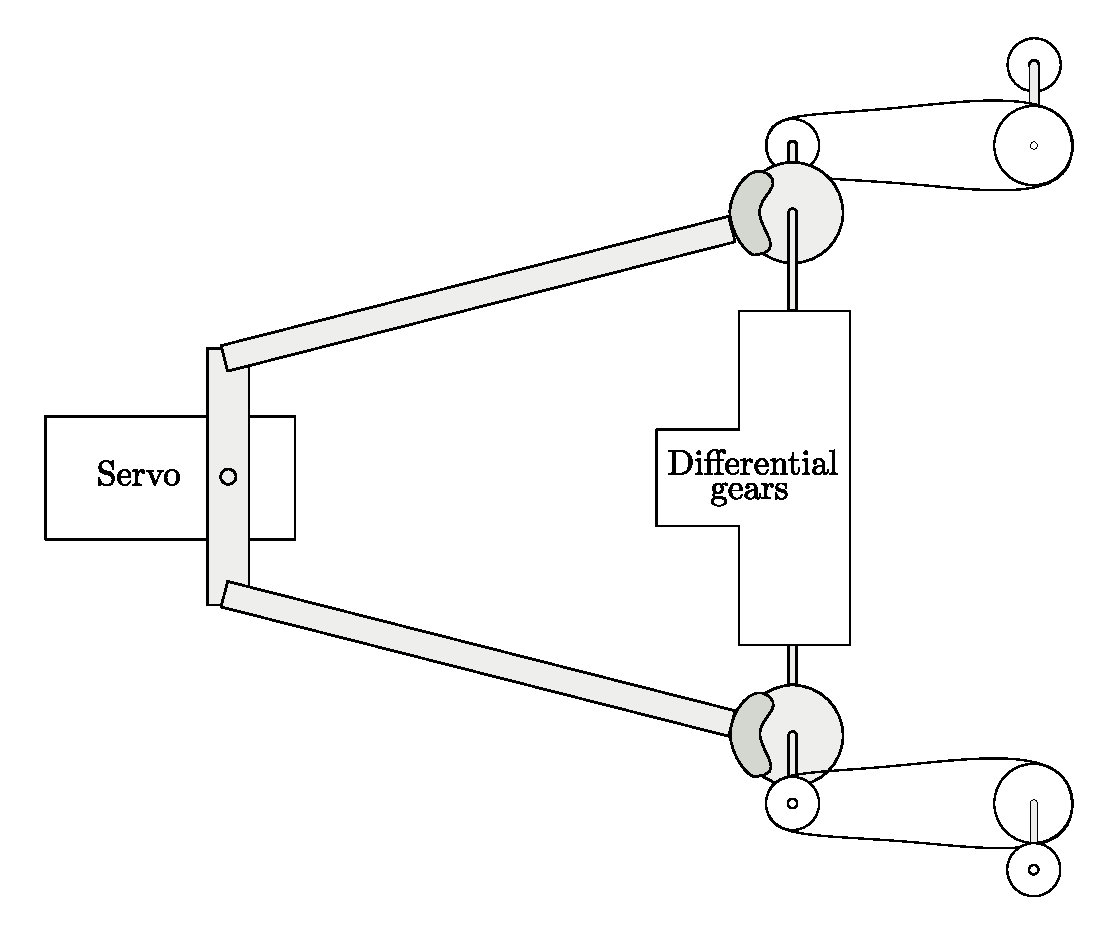
\includegraphics[scale=0.5]{Pictures/steeringMechanical.pdf}
  \end{figure}  
  %\begin{itemize}
   % \item<1-> Example
   % \item<2-> of
   % \item<3-> progressive
   % \item<4-> bullet points
  %\end{itemize}
\end{frame}
%--Next--%
\begin{frame}{Steering Model and Control}{Steering Plant}

    \begin{figure}[H]
    \centering
    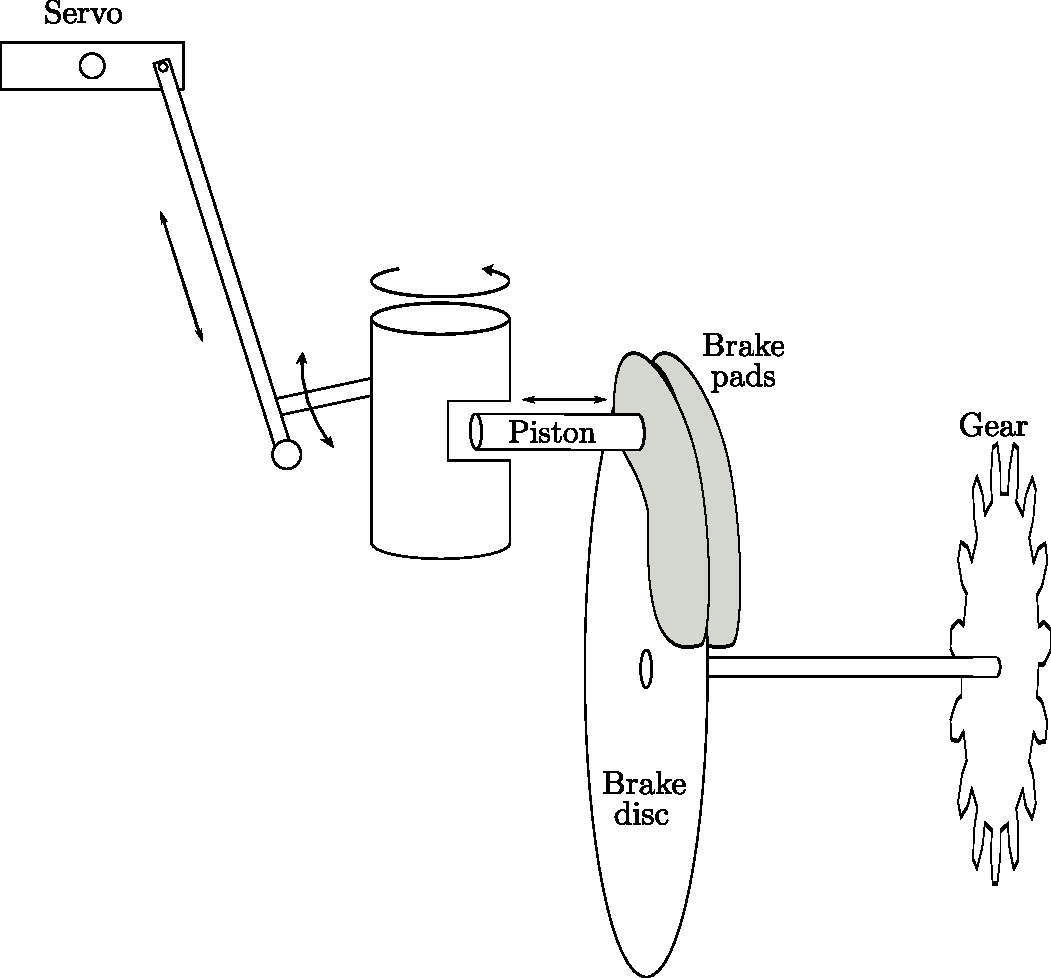
\includegraphics[scale=0.4]{Pictures/brakeDescription.pdf}
  \end{figure}  
\end{frame} 
%%%%%%%%%%%%%%%%

%%%%%%%%%%%%%%%%
\subsection{Directional Model}
%--Next--%
%\begin{frame}{Steering Control of the Vehicle}{Directional Model Enhancement}
%    \begin{block}{Delay}
%      $ U(s) \cdot e^{-\lambda \cdot s} $
%    \end{block}
%    \pause
%    \begin{block}{Padé Approximant}
%        $ e^{-\lambda \cdot s} \simeq \frac{1 - \frac{\lambda}{2} \ \cdot s}{1 + \frac{\lambda}{2} \cdot s} $
%    \end{block}
%    \pause
%    \begin{block}{For small values of lambda (here 30 ms)}
%     $ e^{-\lambda \cdot s} \simeq \frac{1}{1 + \lambda \cdot s} $
%    \end{block}
%\end{frame}
%--Next--%
\begin{frame}{Steering Model and Control}{Directional Model Enhancement}

    \begin{figure}[H]
    \centering
    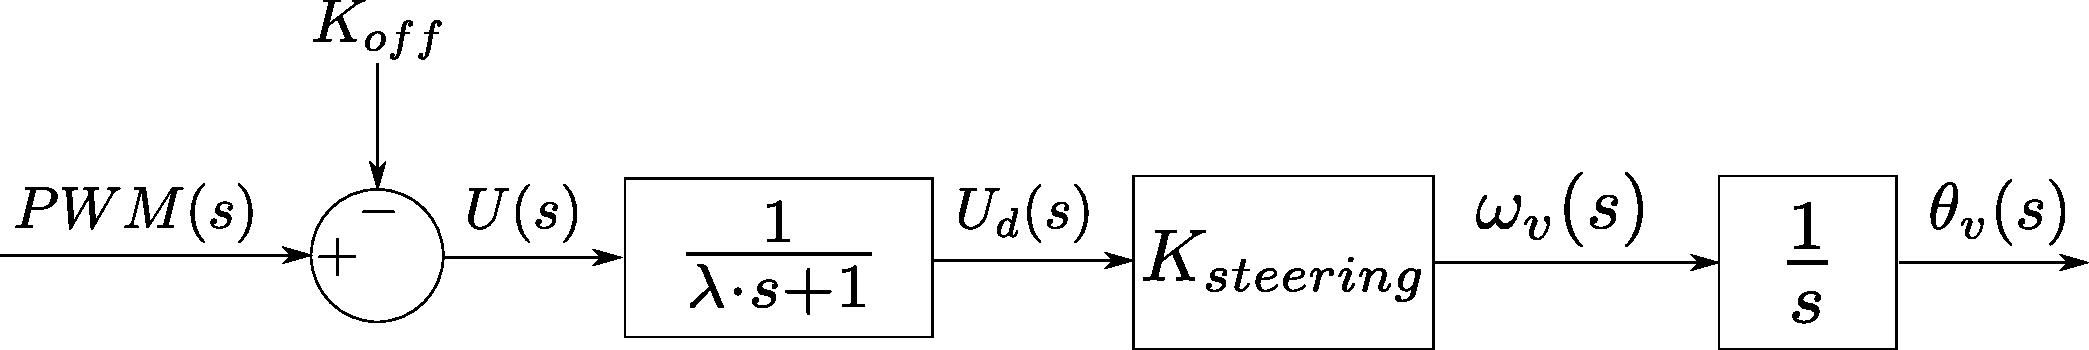
\includegraphics[scale=0.25]{Pictures/basicSteeringModelWithDelay.pdf}
  \end{figure}
\end{frame}
%--Next--%
\begin{frame}{Steering Model and Control}{Directional Model Verification}

    \begin{figure}[H]
    \centering
    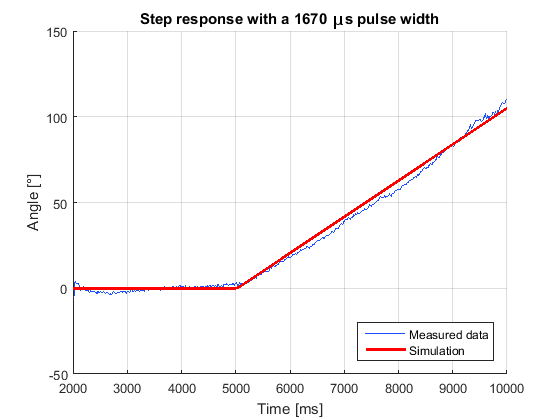
\includegraphics[scale=0.5]{Pictures/plotVerificationSteeringPlant.png}
  \end{figure}
\end{frame}
%--Next--%
\begin{frame}{Steering Model and Control}{Directional Model Verification}

    \begin{figure}[H]
    \centering
    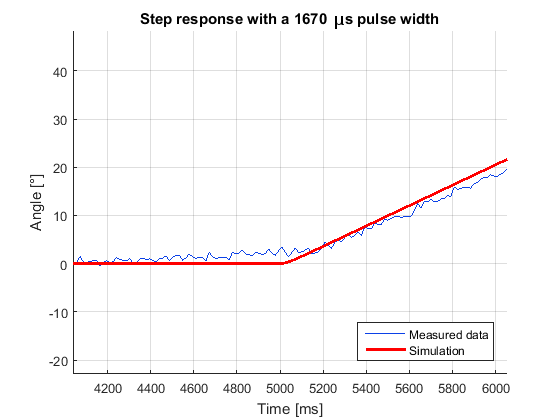
\includegraphics[scale=0.5]{Pictures/plotVerificationSteeringPlantZoom.png}
  \end{figure}
\end{frame}

%%%%%%%%%%%%%%%%

%%%%%%%%%%%%%%%%
\subsection{Directional Control}

%--Directional Controller--%
\begin{frame}{Steering Model and Control}{Directional Controller (P-Controller)}
    \begin{figure}[H]
    \centering
    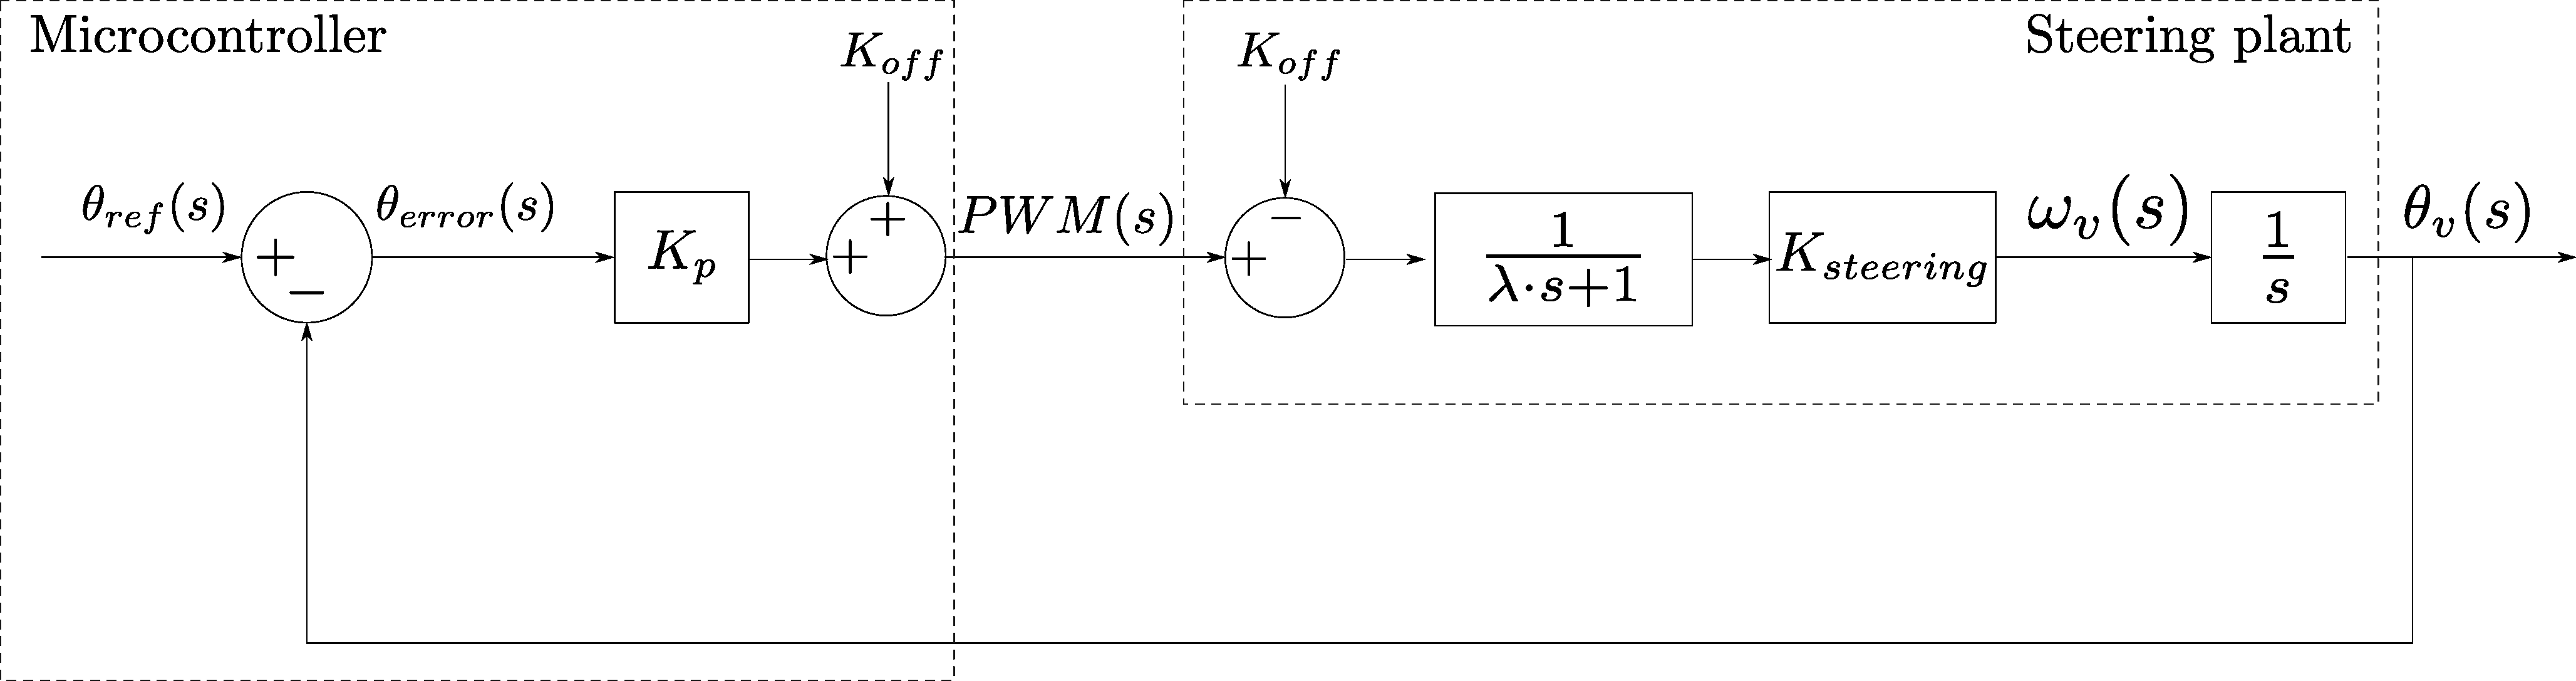
\includegraphics[scale=0.13]{Pictures/basicSteeringModelWithDelayWithFeedback.pdf}
  \end{figure}
\end{frame}

%--Closed-loop TF--%
%\begin{frame}{Steering Control of the Vehicle}{Directional Controller (P-Controller)}
%  \begin{block}{Resulting transfer function}
%    \vspace{4pt}
%    $\frac{\theta_{actual}}{\theta_{wanted}} = \frac{\frac{K_p \cdot K_{steering}}{\left(\lambda \cdot s + 1 \right) \cdot s}}{\frac{K_p \cdot K_{steering}}{\left(\lambda \cdot s + 1 \right) \cdot s} + 1} $
%    \\ \vspace{4pt}
%    \pause
%    …\\\vspace{4pt}
%    $\frac{\theta_{actual}}{\theta_{wanted}} = \frac{K_p \cdot \frac{K_{steering}}{\lambda}}{s^2 + \frac{1}{\lambda} \cdot s + \frac{K_p \cdot K_{steering}}{\lambda}} $ (standard form)
%  \end{block}
%\end{frame}

\begin{frame}{Steering Model and Control}{Directional Controller (P-Controller)}
  \begin{figure}[H]
      \centering
      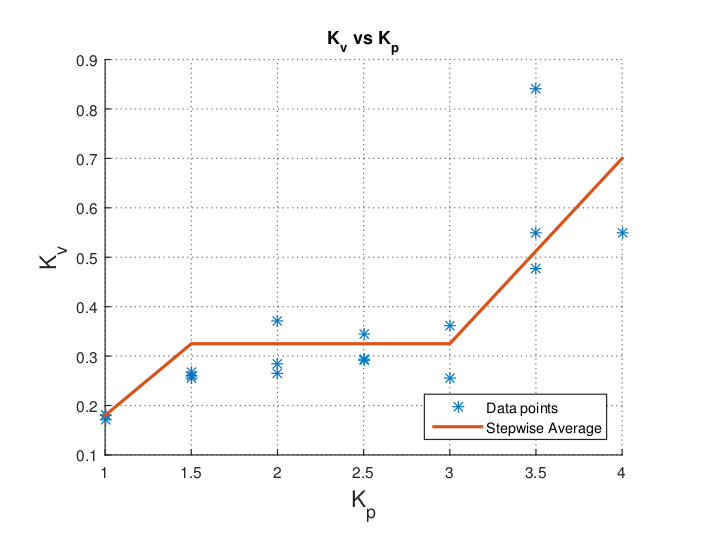
\includegraphics[scale=0.35]{Pictures/KvKpSteeringtest.png}
  \end{figure}
\end{frame}

\begin{frame}{Steering Model and Control}{Directional Controller Verification}
  \begin{figure}[H]
    \centering
    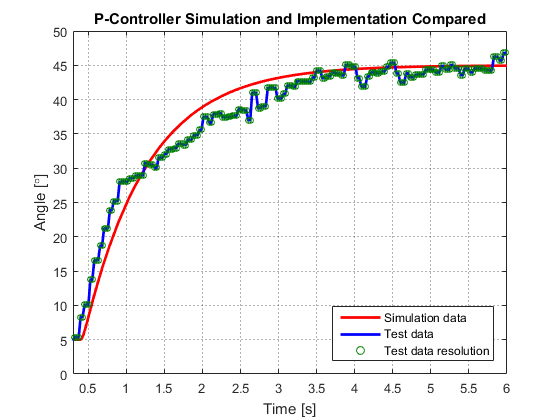
\includegraphics[scale=0.6]{Pictures/SteeringAngularTest.png}
  \end{figure}
\end{frame}

%%%%%%%%%%%%%%%%

%%%%%%%%%%%%%%%%
\subsection{Distance Model}

\begin{frame}{Steering Model and Control}{Line Following}
  \begin{minipage}{\linewidth}
    \begin{minipage}{0.35\linewidth}
      \begin{figure}[H]
        \centering
        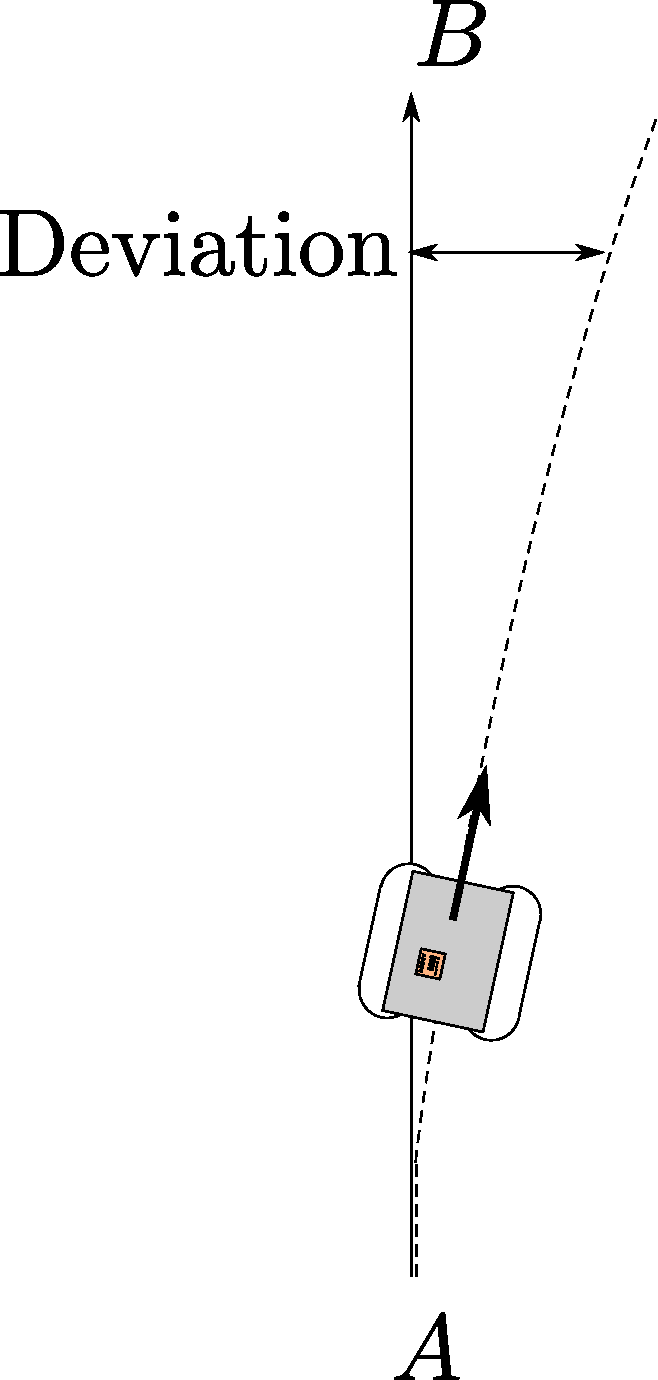
\includegraphics[scale=0.25]{Pictures/vehicleLineDeviation.pdf}
      \end{figure}
    \end{minipage}
    \hspace{0.03\linewidth}
    \begin{minipage}{0.45\linewidth}
      \begin{figure}[H]
        \centering
        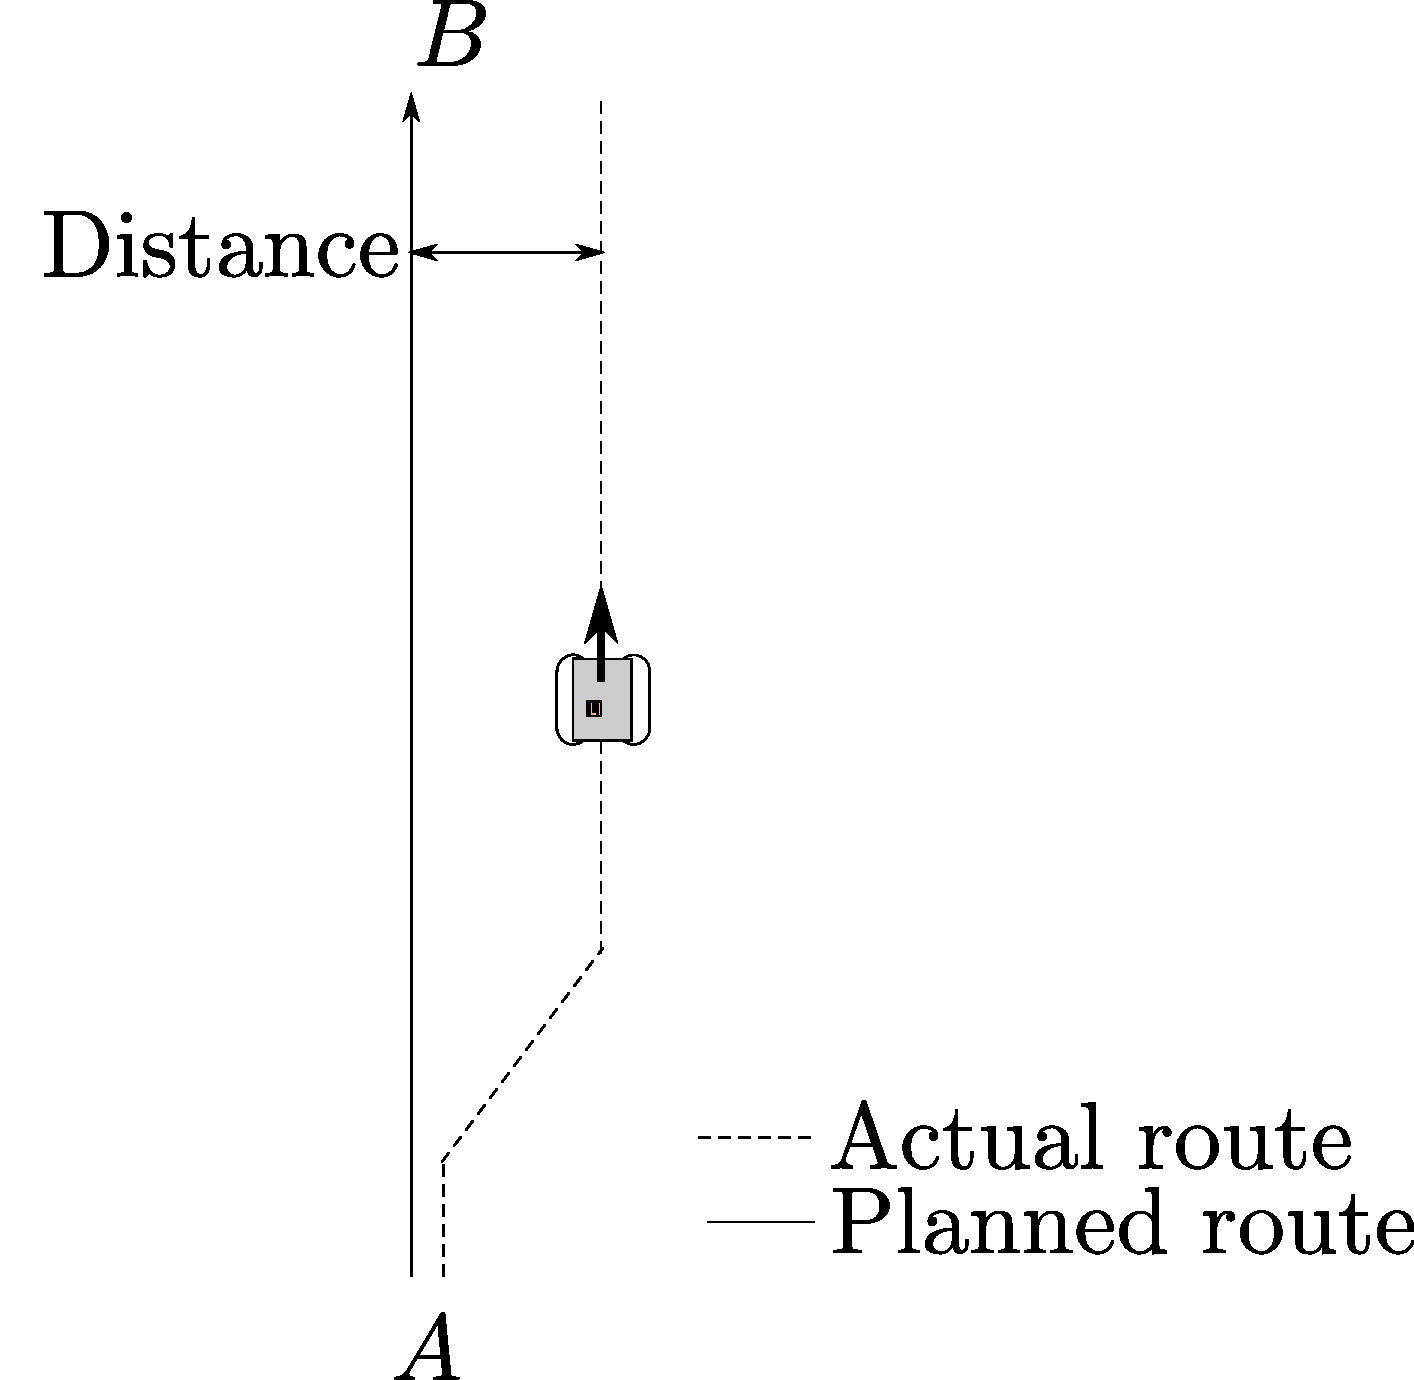
\includegraphics[scale=0.25]{Pictures/steeringDeviation.pdf}
      \end{figure}
    \end{minipage}
  \end{minipage}
\end{frame}

%--Deviation equation --%
%\begin{frame}{Steering Control of the Vehicle}{Distance model}
%  \begin{block}{Deviation equation}
%    \vspace{4pt}
%    $d(t) = v \cdot \int^{t} \sin\left(\Delta\theta (t)\right) \mathrm{d}t $
%    \vspace{4pt}
%    \pause
%  \end{block}
%  \begin{block}{The idea: linearization}
%    $ \Delta\theta \simeq 0 \Rightarrow \sin\left(\Delta\theta\right) \simeq \Delta\theta $ \\
%    \pause
%    $ \vdots $ \\
%    $ D(s)= \frac{\pi}{180} \cdot v \cdot \frac{1}{s} \cdot \left(\theta_{v}(s) - \theta_{ref}(s)\right) $
%  \end{block}
%\end{frame}

%--Complete steering model (for simulation)--%
\begin{frame}{Steering Model and Control}{Distance model}

  $ D(s)= \frac{\pi}{180} \cdot v \cdot \frac{1}{s} \cdot \left(\theta_{v}(s) - \theta_{ref}(s)\right) $

  \begin{figure}[H]
    \centering
    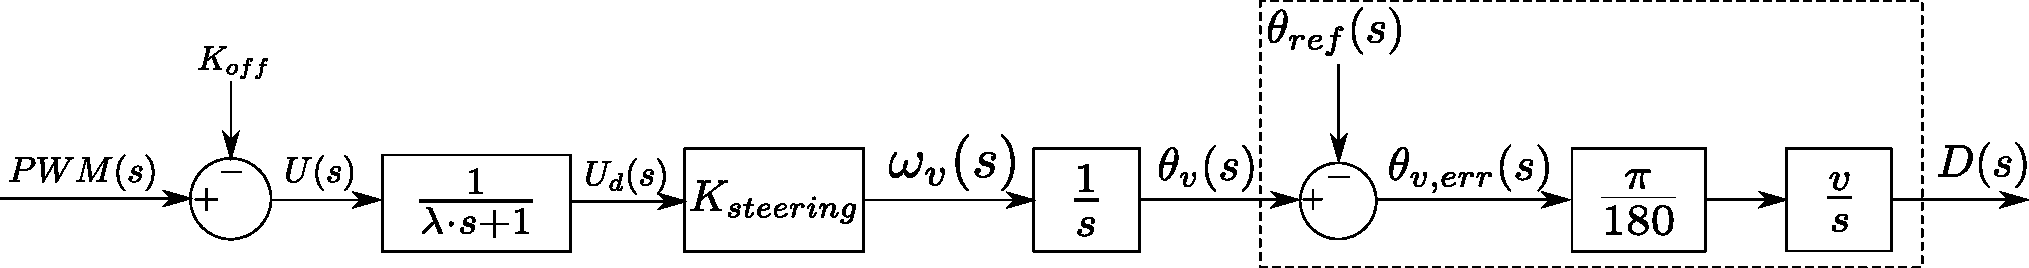
\includegraphics[scale=0.27]{Pictures/steeringModelWithLineFollowing.pdf}
  \end{figure}
\end{frame}

%%%%%%%%%%%%%%%%

%%%%%%%%%%%%%%%%
\subsection{Distance Control}

%--Cascade controller--%
\begin{frame}{Steering Model and Control}{Complete Control}
  \begin{figure}[H]
    \centering
    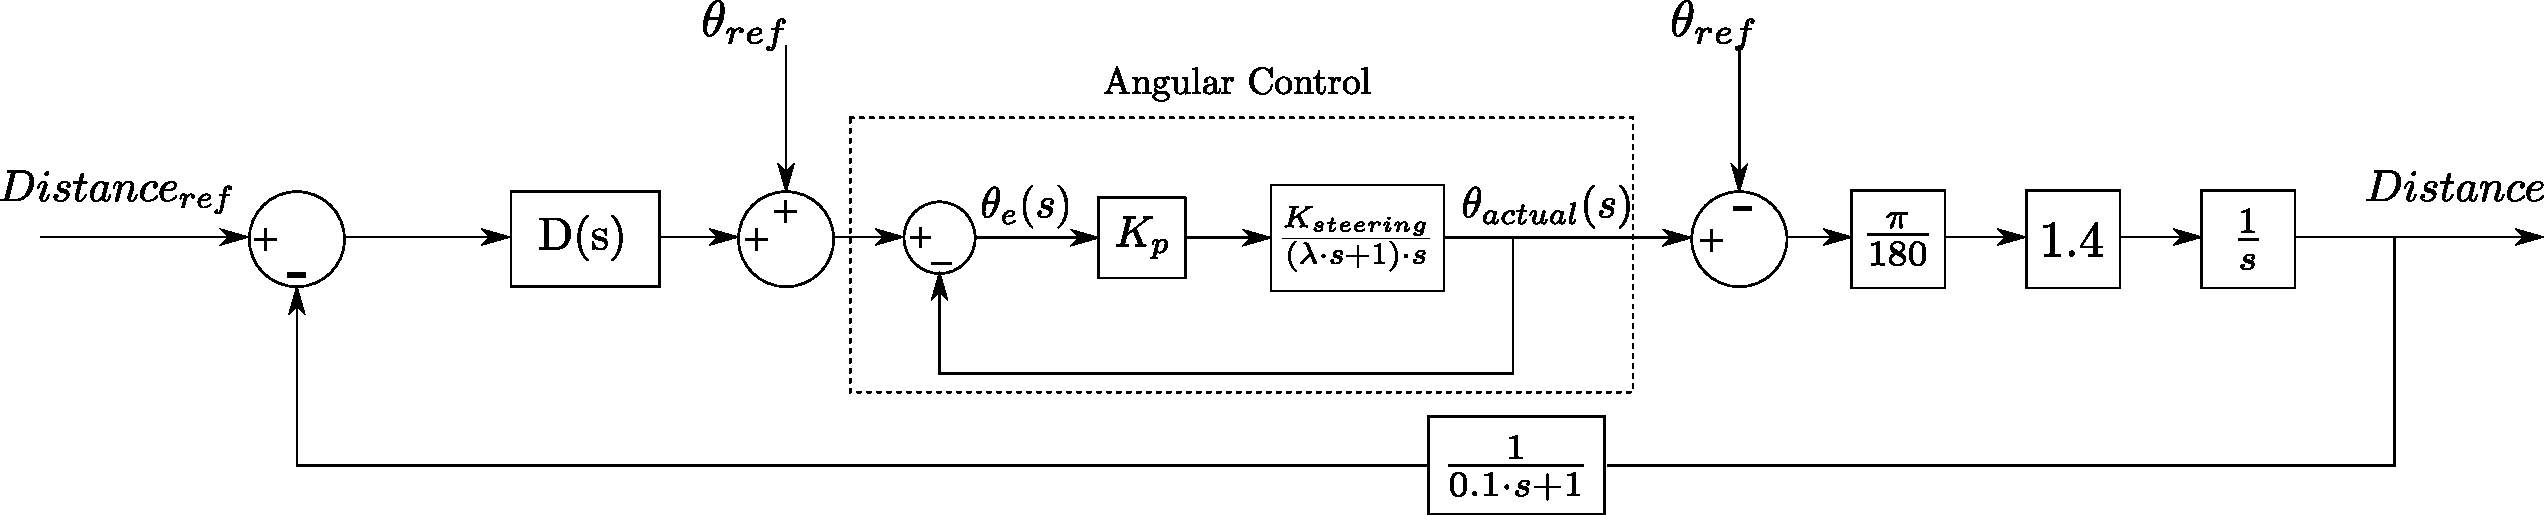
\includegraphics[scale=0.22]{Pictures/steeringBlockCascadeControl.pdf}
  \end{figure}
\end{frame}

%--Step-response P controller (Kp = 1)--%
\begin{frame}{Steering Model and Control}{Distance Control}
  \begin{figure}[H]
    \centering
    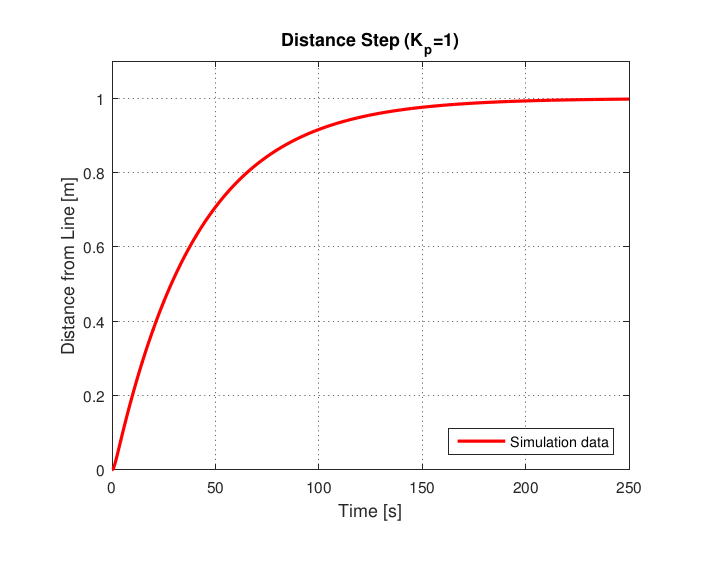
\includegraphics[scale=0.3]{Pictures/distanceStep1.png}
  \end{figure}
\end{frame}

%--Open Loop Bode plot--% 
%\begin{frame}{Steering Control of the Vehicle}{Distance Control}
%  \begin{figure}[H]
%    \centering
%    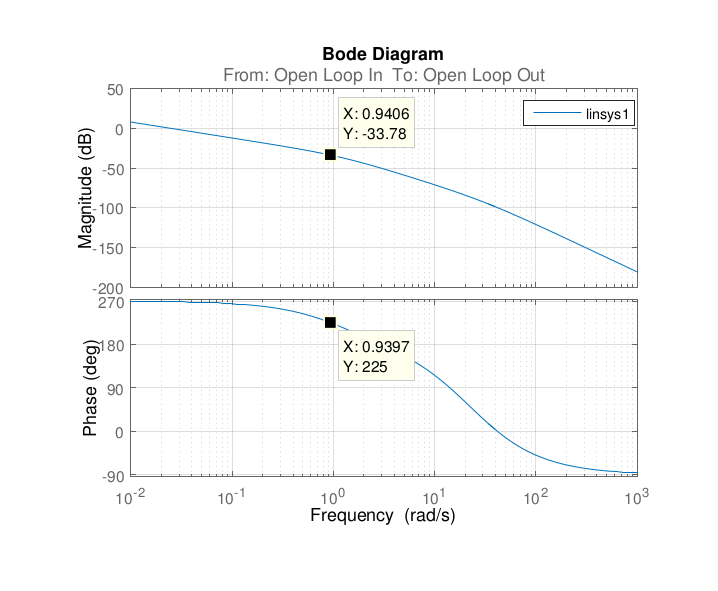
\includegraphics[scale=0.3]{Pictures/distanceBode1.png}
%  \end{figure}
%\end{frame}

%--Step-response P controller (Kp = found value)--%
\begin{frame}{Steering Model and Control}{Distance Control}
  \begin{figure}[H]
    \centering
    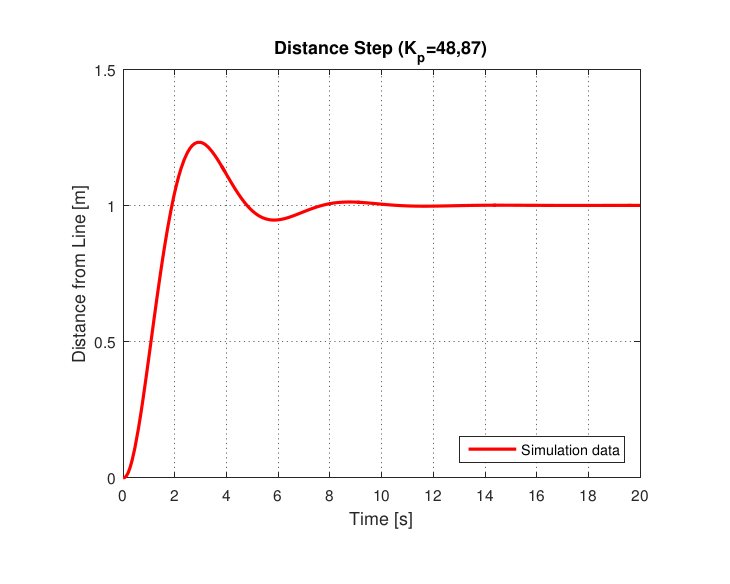
\includegraphics[scale=0.3]{Pictures/distanceStep2.png}
  \end{figure}
\end{frame}

%%--Lead Compensator Design --%
%\begin{frame}{Steering Control of the Vehicle}{Distance Control (Lead Compensator)}
%  \begin{block}{Lead compensator's transfer function}
%    $ D(s) = \frac{1 + a \cdot s}{1 + b \cdot s} = \frac{b}{a} \cdot \frac{\frac{1}{a} + s}{\frac{1}{b} + s}$
%  \end{block}
%  \pause
%  \begin{block}{Design of the lead compensator}
%    \begin{itemize}
%      \item Pole chosen with Nyquist-Shannon sampling theorem
%      $\Rightarrow b = 0,3 > 0,2 $ [s]
%      \item Zero chosen with a compromise (DC gain vs. lead pole) \\
%      $\Rightarrow a = 1 $ [s]
%    \end{itemize}
%  \end{block}
%  \pause
%  \begin{block}{Resulting transfer function}
% $ D(s) = \frac{1 + s}{1 + 0,3 \cdot s} $
%  \end{block}
%\end{frame}

%--Block Diagram with Lead Compensator--%
\begin{frame}{Steering Model and Control}{Distance Control (Lead Compensator)}
  \begin{figure}[H]
    \centering
    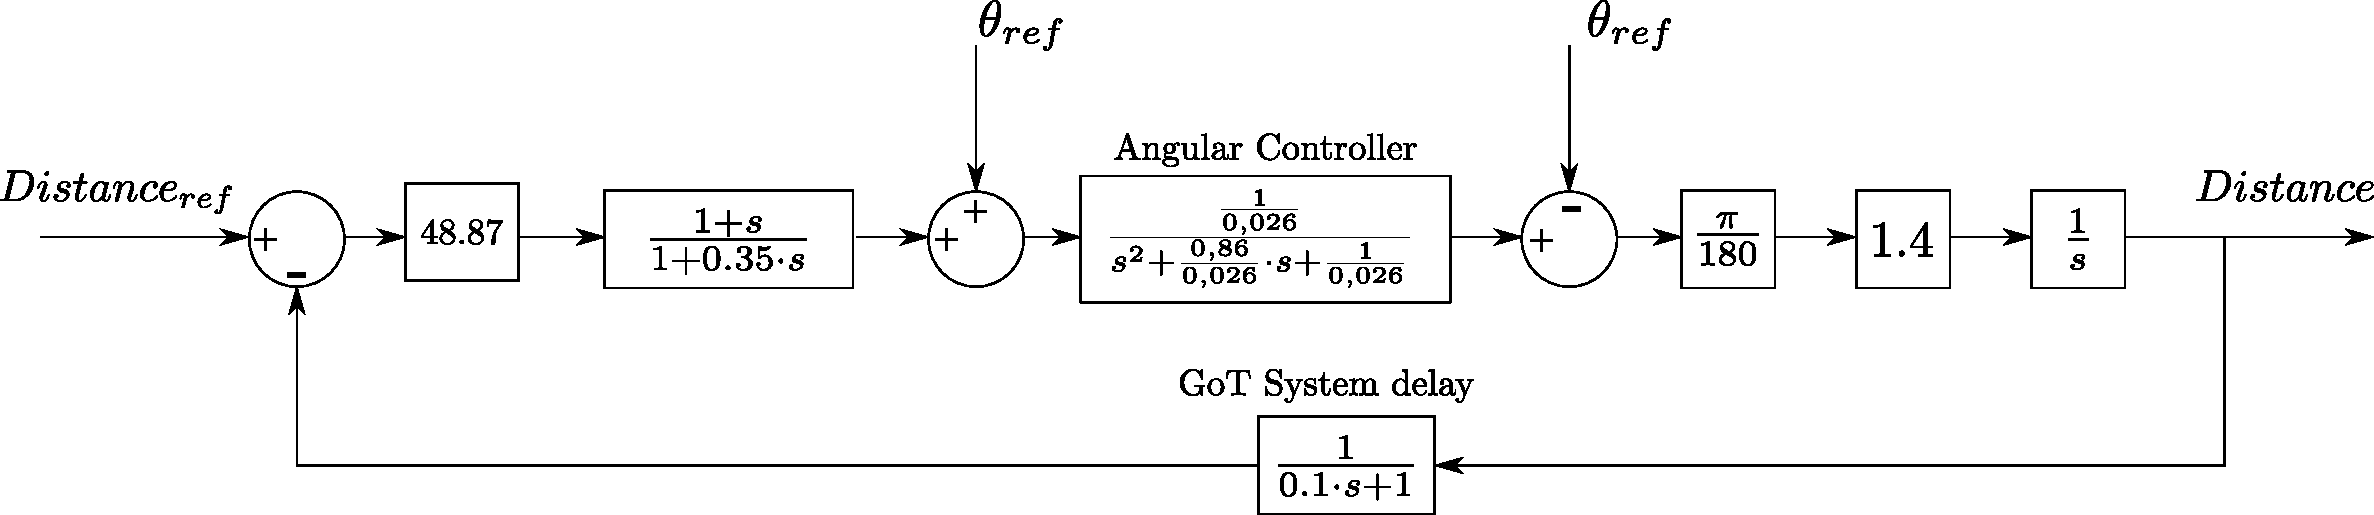
\includegraphics[scale=0.25]{Pictures/finalDistanceController.pdf}
  \end{figure}
\end{frame}

%--Open Loop Bode plot Lead Compensator--% 
%\begin{frame}{Steering Control of the Vehicle}{Distance Control (Lead Compensator)}
%  \begin{figure}[H]
%    \centering
%    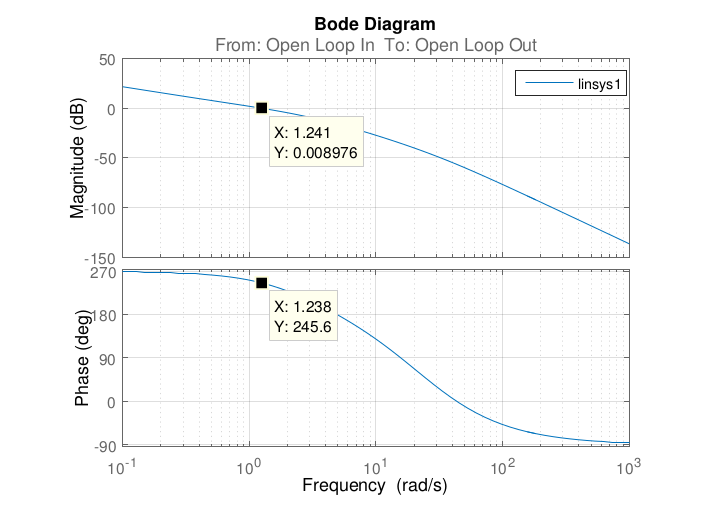
\includegraphics[scale=0.3]{Pictures/distanceBode2.png}
%  \end{figure}
%\end{frame}

%--Step-response with controller (Lead)--%
\begin{frame}{Steering Model and Control}{Distance Control (Lead Compensator)}
  \begin{figure}[H]
    \centering
    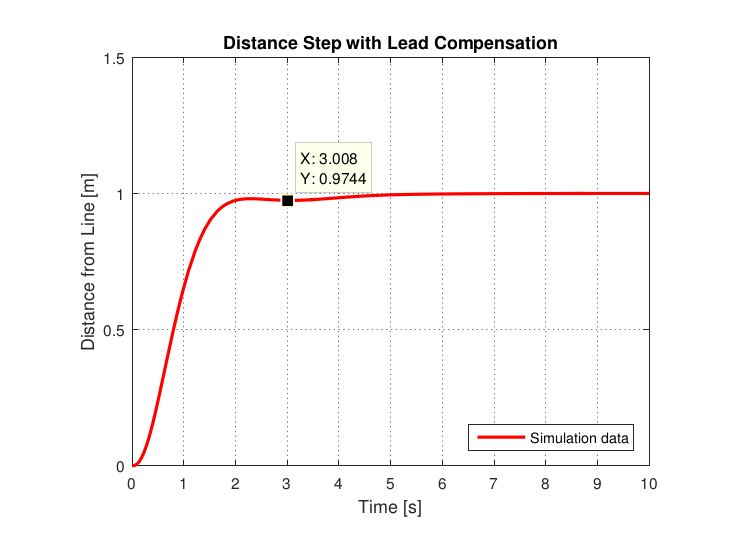
\includegraphics[scale=0.3]{Pictures/distanceStep3.png}
  \end{figure}
\end{frame}

%--Back to reality ! Oh ! there goes gravity !--%
\begin{frame}{Steering Model and Control}{Distance Model in Reality}
    \begin{minipage}{\linewidth}
    \begin{minipage}{0.45\linewidth}
      \begin{figure}[H]
        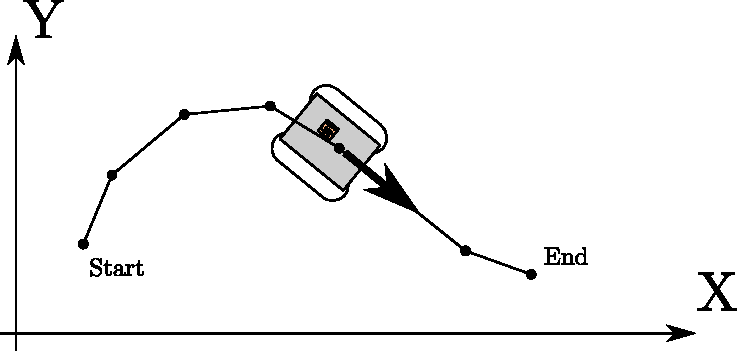
\includegraphics[scale=0.35]{Pictures/stepsGoT.pdf}
        \centering
        %\vspace{-.4cm}
      \end{figure}
    \end{minipage}
    \hspace{0.03\linewidth}
    \begin{minipage}{0.45\linewidth}
      \begin{figure}[H]
        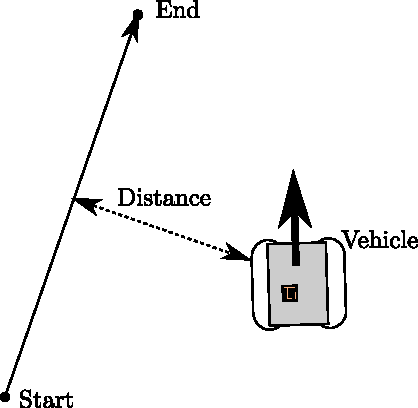
\includegraphics[scale=0.35]{Pictures/DistanceOutLoop.pdf}
        \centering
        %\vspace{-.4cm}
      \end{figure}
    \end{minipage}
  \end{minipage}
\end{frame}